\documentclass[a4paper, 12pt]{article}
\usepackage{listings} 
\usepackage{xcolor}
\usepackage{mdframed}
\usepackage{graphicx}
\definecolor{code-gray}{gray}{0.93}

\begin{document}
\title{ECE 341 - Lab \#2}
\author{Collin Heist}
\date{\today}
\maketitle
\pagenumbering{roman}
\tableofcontents
\lstlistoflistings
\newpage
\pagenumbering{arabic}

\section{Introduction}
The goal of this lab is to practice the methodology of timing processes while using a Micro-controller. For this lab, we'll be using two different methods for time delay. We'll be using a software only method, and a hardware assisted method.

The only new peripheral we'll be using for this lab is the on-board core timer. This is a system timer that increments every two ticks of the system clock. Using the known frequency of the processor, we can figure out how much time has passed by referencing this core timer.

\section{Implementation}
I began using a value of 5,000 for \textbf{COUNTS\_PER\_MS}, and obtained a delay of 565 $\mu$s. Using these two values, I derived that each \textit{count} corresponds to .113 $\mu$s of delay. This led me to test a value of 8,850 which resulted in a delay of 995 $\mu$s. After some more incremental adjustment, I ended with a value of 8,890 and 1.0000 ms of delay.

The code was already provided at the beginning of the lab. The only thing I added was a header file for the main project file \textbf{lab2.h}. The entirety of that code is shown in Listing 1:

	\begin{mdframed}[backgroundcolor=code-gray, roundcorner=10pt,
								innerleftmargin=5, innertopmargin=5, innerbottommargin=5]	
	\begin{lstlisting}[language=C, caption=Project Header File (lab2.h), tabsize=2]
	#ifndef __LAB2_H__
		#define __LAB2_H__

		#define COUNTS_PER_MS 8890
	#endif

	void system_init(void);
	void sw_msDelay (unsigned int mS);
	void hw_msDelay(unsigned int mS);
	\end{lstlisting}
	\end{mdframed}
	
As shown above, the amount of additional code necessary for this lab was quite small. I added the function prototypes, and included safeguards to prevent multiple-inclusion errors. Other than that, I also defined the \textbf{COUNTS\_PER\_MS} macro inside the header file, to avoid any \textit{magic numbers} in my code.

\section{Testing and Validation}
The below table shows how both the software-only and hardware-assisted delays performed over different desired delay times. Clearly, for a longer delay time any discrepancies in the delay calculations become amplified to an extreme amount, so the longer delays (\textgreater100ms) really showcase how precise the delay functions are.
\begin{table}[!h]
\centering
\begin{tabular}{c|c|c}
\textbf{Desired Delay} & \textbf{Measured (Software)} & \textbf{Measured (Hardware)} \\
\hline
1 ms & 0.9922 ms & 1.000 ms \\
10 ms & 10.044 ms & 10.000 ms \\
100 ms & 100.276 ms & 100.000 ms \\
1000 ms & 1000.960 ms & 999.000 ms \\
\end{tabular}
\caption{Desired vs. measured delay of both delay functions}
\end{table}

Based on these results, it is quite clear that the primary source of error lies in the software-only delay function, and almost certainly with my choice of the delay counting variable. Based off the nature of the micro-controller, it is very unlikely that any integer value would give a perfect one millisecond delay, and clearly my choice was off by a small amount. Despite this, the value I chose was close enough that over 1000ms the error was still less than 1 millisecond in total (below .1\% error). Even though I did not record any error for the hardware-assisted delaying function, it's likely that's not exact as well. Over an even longer amount of time, I'd make a presumption that errors would arise. My suspicion is that this would be a result of the imprecision of the on-board clock.

\section{Questions}
There are no questions provided for this lab.

\section{Conclusion}
When it comes to timing, the Micro-controller is quite limited. Being disconnected from the Internet (at least for now) makes reliably timing a task quite a bit more difficult than I would have foreseen. We're quite limited in many aspects with timing.

In some instances, a software-only delay would be a sufficient enough tool. An instance of this would be tasks where the speed of the processor is precisely known beforehand, such that a 'counter' can be consistent enough to use for timing mechanisms. In this instance, software-only timing is easier to implement than its hardware-assisted counterpart. In contrast, a situation where the exact processor speed is \textit{not} known allows for the use of such hardware-assisted delays. This type of timer is practically guaranteed to be accurate (depending on the quality of the on-board clock for the micro-controller).

The benefits of these delays are that they both work. Perhaps they require a bit of fiddling or characterization of the processor, but it makes accurate time measurement and delays very possible with limited resources. A \textbf{huge} downside of these delays is that they're \textit{blocking} functions, meaning that no code can be performed in parallel to these while the delay is being performed. This means that any additional tasks that the processor needs to perform are required to wait until the delay is over.

The limitations of these delays depends on the resources that they utilize. For example, the software-only implementation currently uses an unsigned integer as a parameter to determine how many milliseconds to wait. Without refactoring the code to utilize floating point numbers, the \textit{smallest} time that can be delayed is one millisecond. And the \textit{largest} time is 4,294,967,295 milliseconds (the largest number that is representable using a 32-bit unsigned int), or approximately 7.101 weeks.

For the hardware assisted delay, since this function \textit{also} utilizes an unsigned integer as it's parameter to determine how long to wait, the function has to wait at least one millisecond. But the maximum wait time for this function is quite a bit smaller due to the calculation of unsigned int tWait. This variable can be a maximum of 4,294,967,295, yet due to the value of CORE\_MS\_TICK\_RATE, the largest possible mS (i.e. delay) that can achieve this is calculated with $$2^{32}-1=CORE\_MS\_TICK\_RATE*max\_delay$$ If a value of 80 MHz is used, then divided by 2000 to calculate \linebreak CORE\_MS\_TICK\_RATE, then the maximum delay is thus 107,374 milliseconds (about 1.79 minutes).

As mentioned before, by refactoring these delay functions to accept a floating point number as a parameter, rather than just unsigned integers, the range of the delay could be vastly increased. If the maximum delay period was the only concern.. for the hardware-assisted function (it might seem counter-intuitive), a \textit{slower} processor could achieve a longer maximum delay. 

\section{Attachments}
\begin{figure}[htp]
\centering
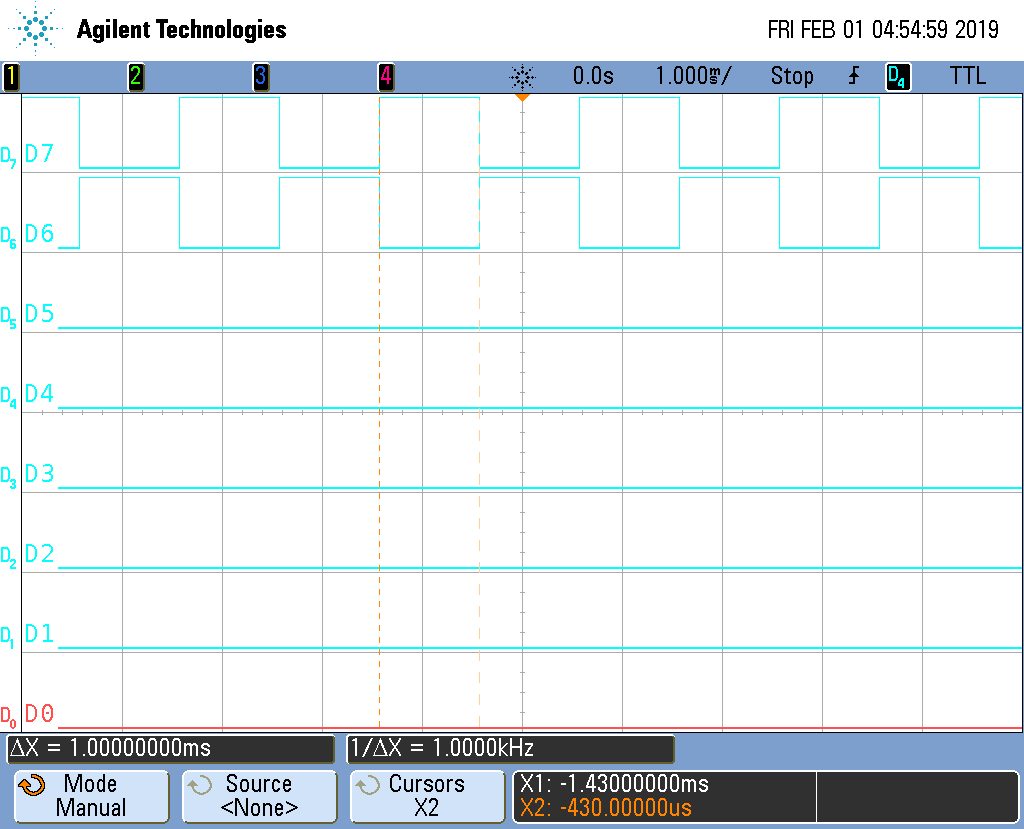
\includegraphics[width=.8\textwidth]{1ms_hardware.png}
\caption{The 1 ms hardware-assisted delay}
\end{figure}

\begin{figure}[p]
\centering
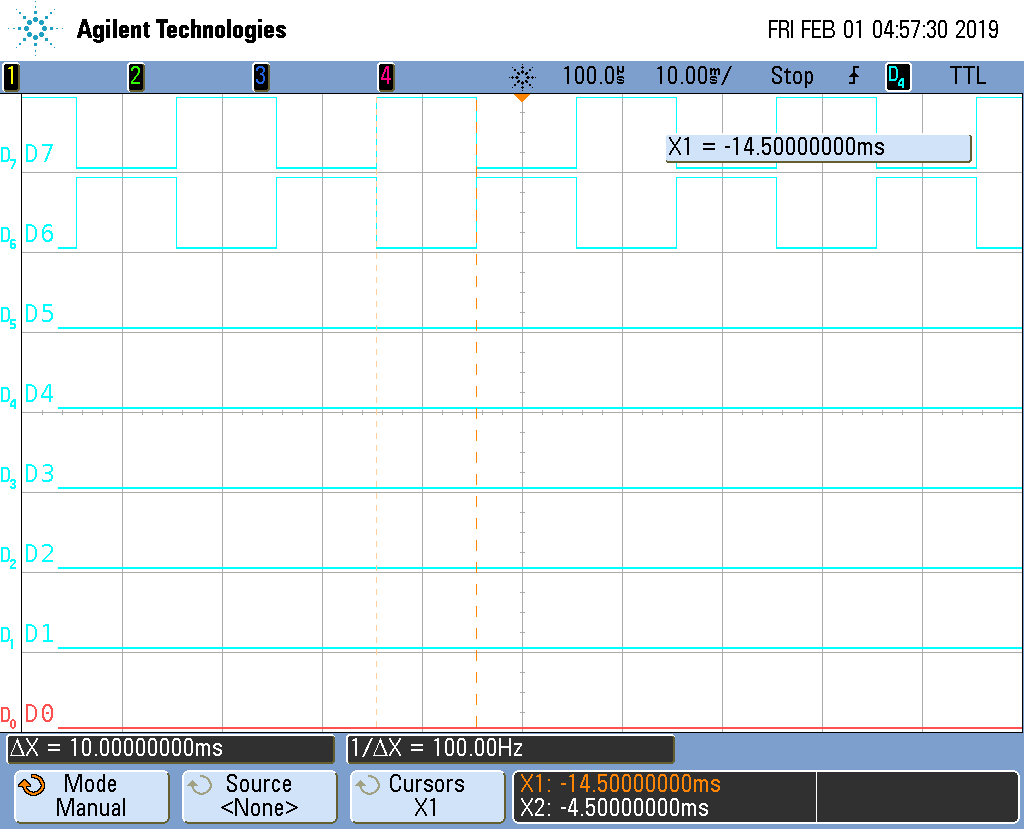
\includegraphics[width=.8\textwidth]{10ms_hardware.png}
\caption{The 10 ms hardware-assisted delay}
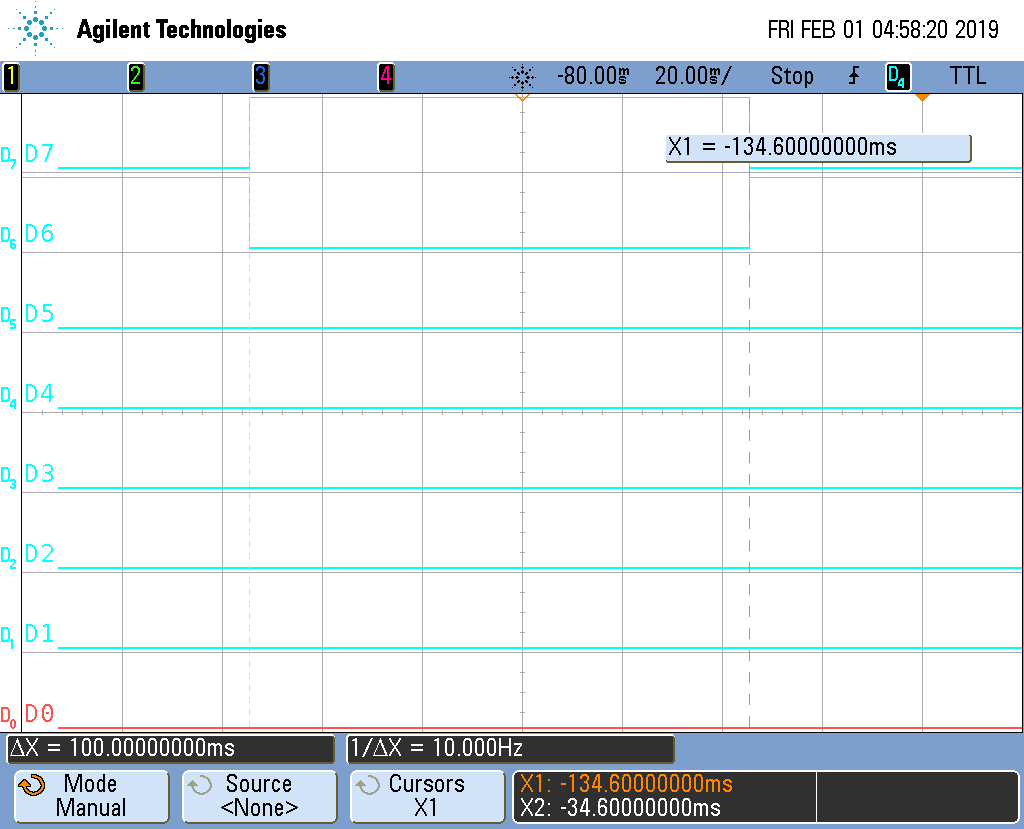
\includegraphics[width=.8\textwidth]{100ms_hardware.png}
\caption{The 100 ms hardware-assisted delay}
\end{figure}

\begin{figure}[p]
\centering
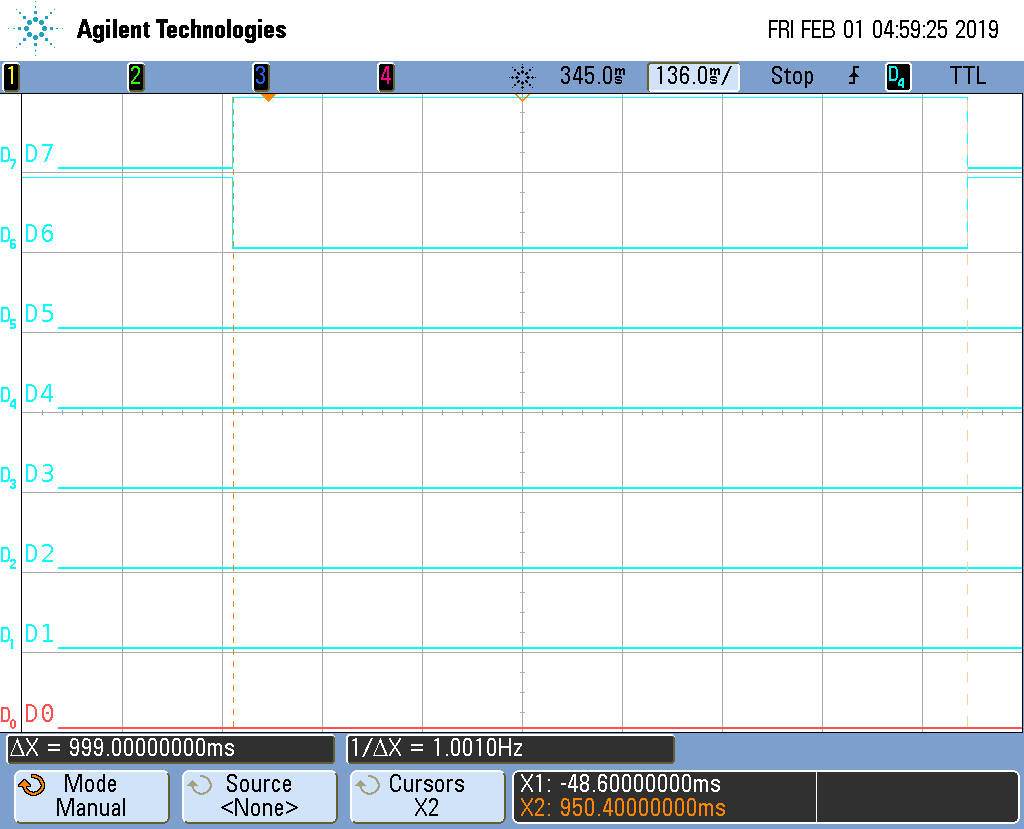
\includegraphics[width=.8\textwidth]{1000ms_hardware.png}
\caption{The 1000 ms hardware-assisted delay}
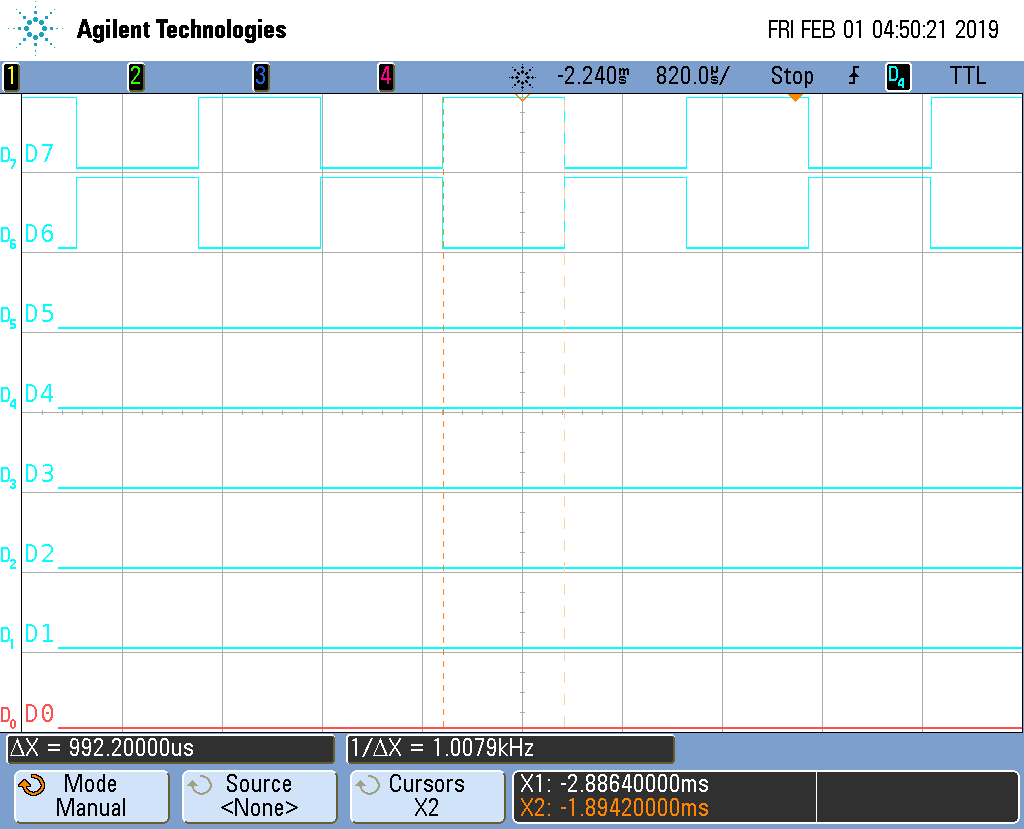
\includegraphics[width=.8\textwidth]{1ms_software.png}
\caption{The 1 ms software-only delay}
\end{figure}

\begin{figure}[p]
\centering
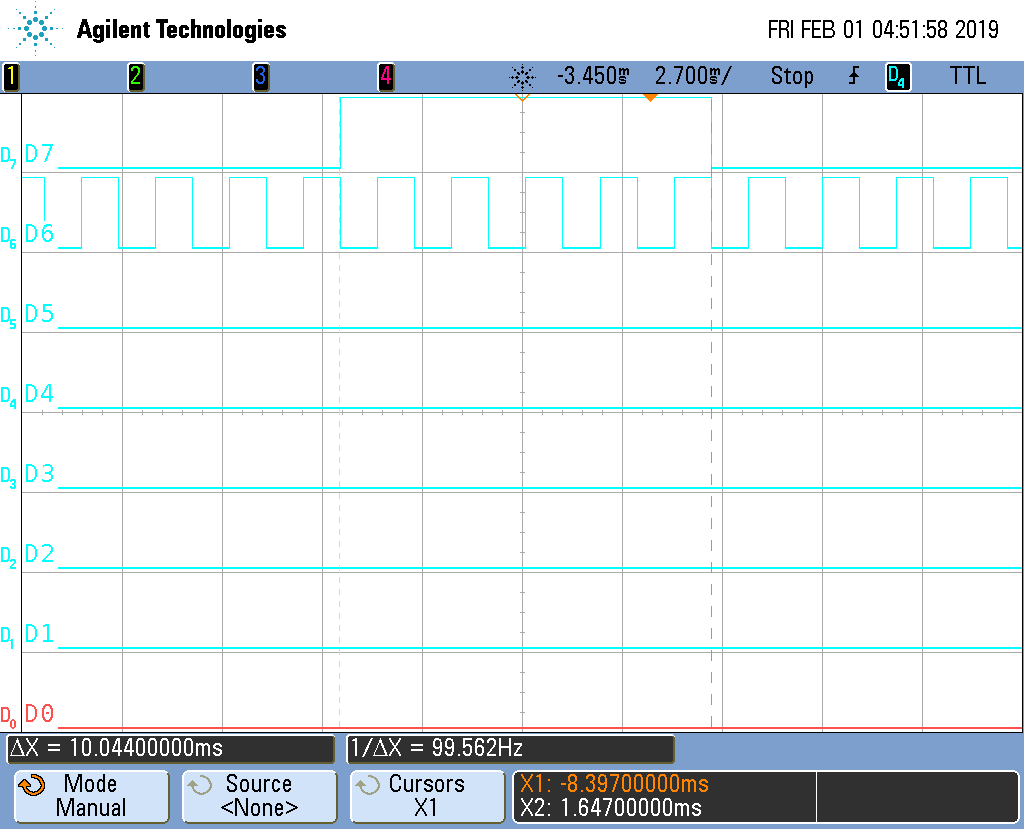
\includegraphics[width=.8\textwidth]{10ms_software.png}
\caption{The 10 ms software-only delay}
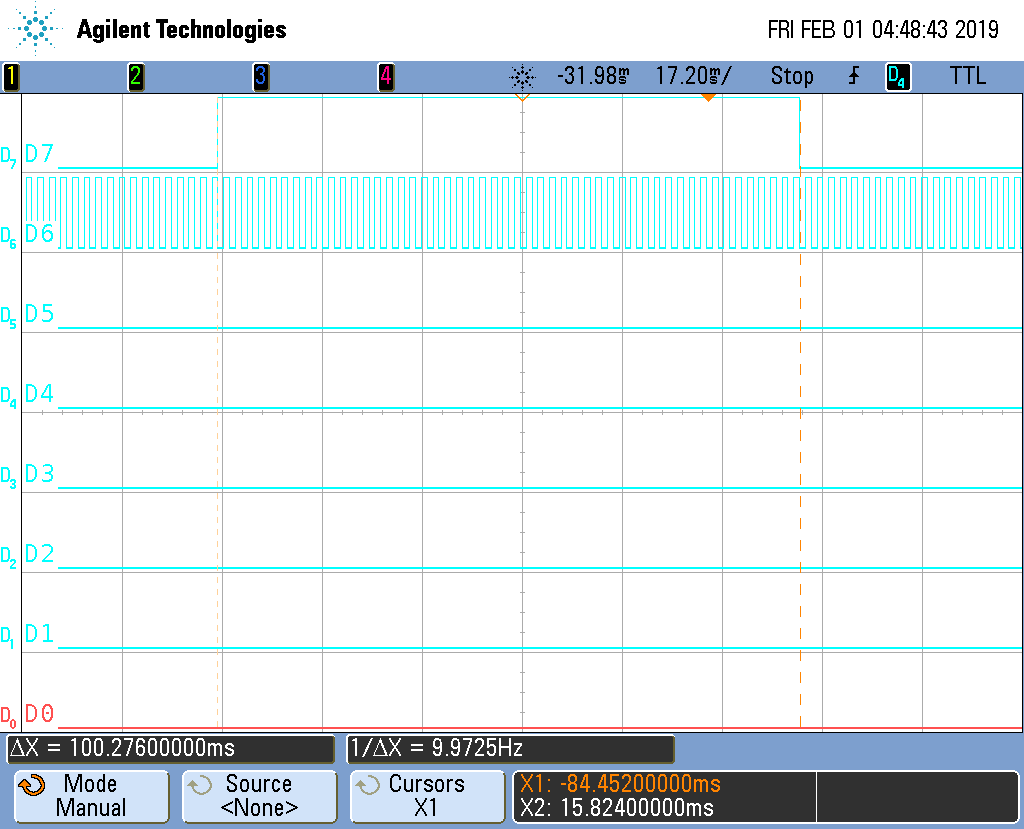
\includegraphics[width=.8\textwidth]{100ms_software.png}
\caption{The 100 ms software-only delay}
\end{figure}

\begin{figure}[htp]
\centering
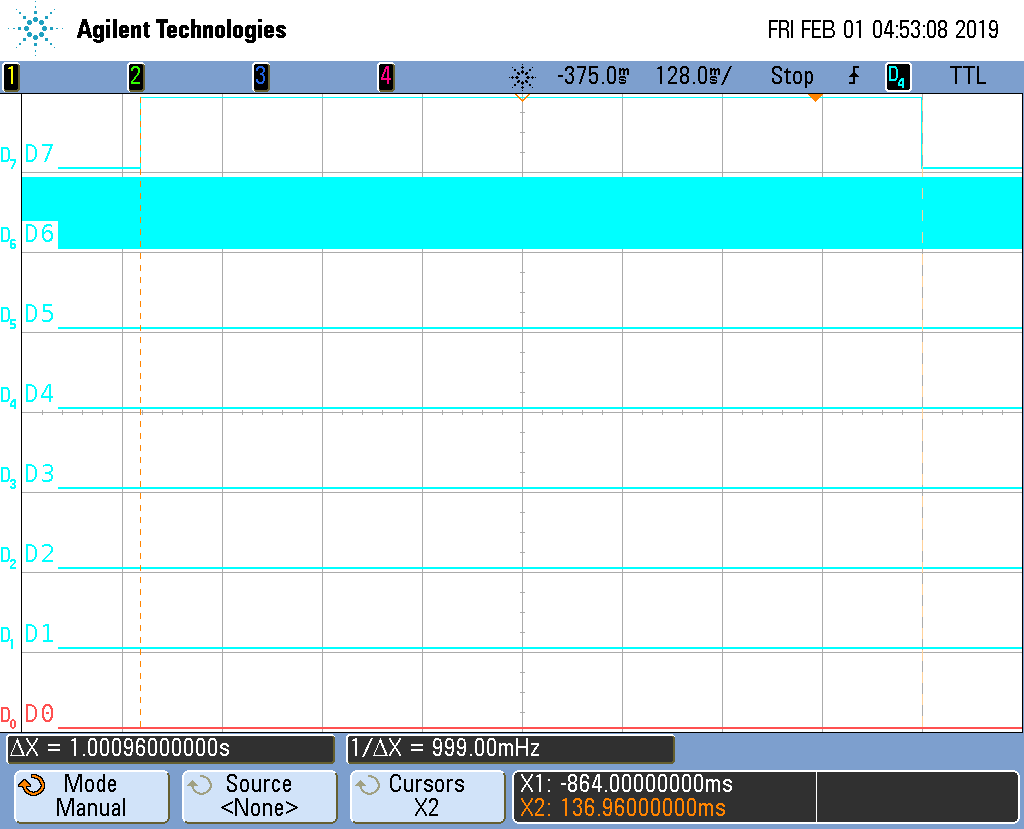
\includegraphics[width=.8\textwidth]{1000ms_software.png}
\caption{The 1000 ms software-only delay}
\end{figure}

\end{document}